\section{Concurrency}\label{sec:concurrency}
The term concurrency is a general term for ways a computer system performs multiple tasks simultaneously. It covers the \textit{simulation} of multiple tasks running at the same time through process switching, as well as work done in parallel. To disambiguate, based on the definition:

\blockcquote{Bryant2016}{We use the term concurrency to refer to the general concept of a system with multiple, simultaneous activities, and the term parallelism to refer to the use of concurrency to make a system run faster.}

We infer that parallelism is a type of concurrency to speed up the system, while concurrency, in general, may have purposes not related to speed, for example, synchronization of tasks.

Concurrency is a complex, large, and hardware-dependent subject~\cite{Sebesta2016}. The limitations of the Arduino hardware concerning concurrency, specifically the \gls{cpu}, are explored before concurrency in general because the project is, first and foremost, about programming language design - not concurrency.

\subsection{Arduino hardware}\label{subsec:arduinohardware}
The Arduino Uno board uses the ATmega328P microcontroller~\cite{ArduinoUno}. The architecture of this microcontroller is a scalar single-core processor without hyperthreading(intel) or \gls{smt} (AMD) equivalents~\cite{ATmega328P}.

Since there is only a single core that does not contain any duplicate copies of CPU hardware (for multithreading), the only hardware parallelism on the Arduino Uno is instruction-level parallelism, and only to the level of up to 1 instruction per clock cycle (scalar). This parallelism is also handled directly by the \gls{cpu} and does not impact the instruction set available to developers.


\begin{figure}[htb!]
    \centering
    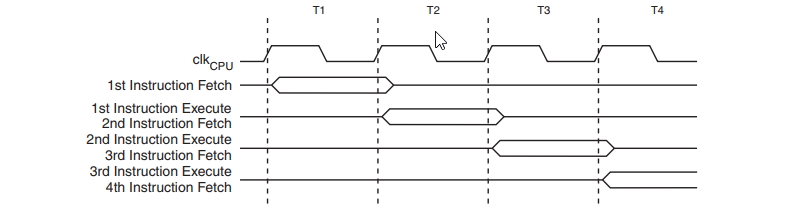
\includegraphics[width=\textwidth]{figures/Arduino_Pipeline.png}
    \caption{The parallel intruction fetches and intruction executions \cite{ATmega328P}}
    \label{fig:arduinopipeline}
\end{figure}


Therefore, the Arduino is a uniprocessor~\cite{Bryant2016} whose architecture does not support parallel processing - and for the remainder of the report, the term concurrency refers to concurrency \textbf{without parallelism}.

Even unicore processors can support several models for concurrency at the application software level, which makes sense since most computers often have more processes running than \glspl{cpu}. Achieving this concurrency is done through interleaving instructions of different processes, which lets the \gls{cpu} appear to run multiple programs.

This interleaving is commonly handled by an \gls{os}, which manages the hardware resources~\cite{Bryant2016}. However, by default, the Arduino does not have an \gls{os}. It is still possible to achieve concurrency on an Arduino, but not without a scheduler or scheduling.

\subsection{Concurrency on an Arduino}\label{subsec:concurrencyinarduino}
\todo{Titlen passer ikke til sektionen: Otherways to achieve concurrency on arduino?}
\todo{Måske gøre det mere tydeligt at hvad pointen er med de to funktioner. Vi læste det og fangede ikke pointen før vi læste andengang}
The scheduler is the part of the \gls{os} that handles the planning and switching of different tasks on the CPU within the system. However, an \gls{os} is not the only way to obtain scheduling behavior. Several online tutorials~\cite{BadExample1, BadExample2} demonstrate different techniques to achieve concurrency on an Arduino, such as using the Arduino functions millis() and interrupt().

The millis() technique executes different pieces of code depending on some programmer-defined timeslices and comparisons between the current time and an earlier time. The interrupt() method uses the \gls{cpu} interrupt command to interrupt the \gls{cpu} and restart it from another place in the code.

Both methods require the programmer to think deeply about how they wish for the program to execute, which can get complicated and frustrating fast. The interrupt() case is a very low-level command that might not work entirely as a novice or hobbyist expects. In the case of the millis() method, it requires many global variables to execute the program correctly, which can be difficult. In both cases, the code may be hard to maintain or understand.

These examples highlight a general difficulty with the Arduino model, and several solutions to the described problems exist, some of which are explored in the next section.
